\documentclass[11pt,a4paper]{article}

\usepackage[utf8]{inputenc}
\usepackage[T1]{fontenc}
\usepackage{lmodern}
\usepackage[french]{babel}
\usepackage[margin=2.4cm]{geometry}
\usepackage{microtype}
\usepackage{booktabs}
\usepackage{array}
\usepackage[table]{xcolor}
\usepackage{amsmath}
\usepackage{amssymb}
\usepackage{mathtools}
\usepackage{enumitem}
\usepackage[most]{tcolorbox}
\usepackage{tabularx}
\usepackage{caption}
\usepackage{titlesec}
\usepackage[section]{placeins}
\usepackage{hyperref}

\definecolor{navy}{HTML}{1F3864}
\definecolor{bluemid}{HTML}{2E5496}
\definecolor{lightblue}{HTML}{D6E0F0}
\definecolor{accent}{HTML}{C0491F}

\hypersetup{colorlinks=true, linkcolor=bluemid, urlcolor=bluemid,
  pdftitle={Note - Vasicek dirige pour les piliers DORA},
  pdfauthor={Kelian Kaddouri}}

\newtcolorbox{cle}[1][]{colback=lightblue!40,colframe=navy,boxrule=0.6pt,
  arc=2pt,left=8pt,right=8pt,top=6pt,bottom=6pt,before skip=9pt,after skip=9pt,#1}
\newtcolorbox{attention}[1][]{colback=accent!8,colframe=accent,boxrule=0.6pt,
  arc=2pt,left=8pt,right=8pt,top=6pt,bottom=6pt,before skip=9pt,after skip=9pt,#1}

% mise en page : titres, legendes, flottants
\titleformat{\section}{\normalfont\large\bfseries\color{navy}}{\thesection}{0.6em}{}
\titlespacing*{\section}{0pt}{1.9ex plus .3ex minus .2ex}{1.0ex plus .2ex}
\captionsetup{font=small,labelfont={bf,color=navy},labelsep=period,skip=6pt}
\renewcommand{\topfraction}{0.92}
\renewcommand{\bottomfraction}{0.85}
\renewcommand{\textfraction}{0.07}
\renewcommand{\floatpagefraction}{0.75}
\setcounter{topnumber}{3}

\newcommand{\Y}{Y}
\newcommand{\eps}{\varepsilon}

\title{\vspace{-1.2cm}\color{navy}\bfseries Vers un Vasicek dirigé pour les piliers DORA\\[2pt]
  \large Note pédagogique : la structure systémique dépend du pilier}
\author{Kélian Kaddouri}
\date{\today}

\begin{document}
\maketitle
\vspace{-0.6cm}

\begin{cle}
\textbf{Le fil de la note.} On part du modèle de Vasicek standard (un seul facteur
systémique, une seule corrélation), on l'ouvre en \textbf{deux temps} : \emph{(A)} chaque
pilier DORA reçoit \textbf{son propre} facteur systémique et sa propre sensibilité :
la structure systémique \textbf{dépend du pilier~$j$} ; \emph{(B)} les piliers se
propagent l'un l'autre de façon \textbf{dirigée} (asymétrique). Le seuil de déclenchement
$K_j$ n'est plus $\Phi^{-1}(\mathrm{PD})$ mais un seuil \textbf{réglementaire calibré}.
\end{cle}

\section{Le point de départ : le Vasicek à un facteur}

Pour une entité~$i$ (à l'origine : un emprunteur), on écrit une \textbf{variable latente},
une \og{}santé\fg{} non observée :
\begin{equation}
X_i \;=\; \sqrt{\rho}\;\Y \;+\; \sqrt{1-\rho}\;\eps_i .
\end{equation}
Chaque terme a un sens précis :
\begin{itemize}[leftmargin=1.4em,itemsep=1pt]
\item $\Y \sim \mathcal N(0,1)$ : le \textbf{facteur systémique}, commun à \emph{toutes}
  les entités (le \og{}temps qu'il fait\fg{} sur le marché). Une mauvaise réalisation de
  $\Y$ fragilise tout le monde en même temps.
\item $\eps_i \sim \mathcal N(0,1)$ : le \textbf{choc idiosyncratique}, propre à~$i$ et
  indépendant du reste.
\item $\rho \in [0,1]$ : la \textbf{part du systémique}. Plus $\rho$ est grand, plus les
  entités bougent ensemble. C'est \emph{la même valeur pour tout le monde}.
\end{itemize}
L'incident (à l'origine : le défaut) se produit quand la santé passe sous un \textbf{seuil} :
\begin{equation}
D_i = 1 \iff X_i < K_i, \qquad\text{avec, dans le modèle classique,}\quad
K_i = \Phi^{-1}(\mathrm{PD}_i).
\end{equation}

\begin{attention}
\textbf{Deux hypothèses de ce modèle sont fausses pour le cyber/DORA.}
\emph{(1)} La dépendance y est \textbf{symétrique} (un seul $\Y$, un seul $\rho$) : elle ne
peut pas dire \og{}P1 entraîne P2 plus que l'inverse\fg{}. Or nos données sont dirigées à
\textbf{81\,\%}. \emph{(2)} Le seuil $K_i=\Phi^{-1}(\mathrm{PD}_i)$ suppose une PD stable et
mesurable, et une \og{}valeur de firme\fg{} sous-jacente : rien de tout cela n'existe en cyber.
\end{attention}

\section{Généralisation A : la structure systémique dépend de l'entité \emph{et} du pilier}

On indexe désormais par \textbf{(entité~$i$, pilier~$j$)}, avec $j\in\{1,\dots,5\}$ les cinq
piliers DORA. L'idée centrale de cette note :

\begin{cle}
\textbf{Chaque pilier a sa propre \og{}météo systémique\fg{}, et chaque entité y est plus ou
moins exposée.} On remplace le facteur unique $\Y$ par \textbf{un facteur par pilier} $\Y_j$,
et la corrélation unique $\rho$ par une sensibilité $\rho_{ij}$ \textbf{propre à l'entité et
au pilier} :
\end{cle}

\begin{equation}
\boxed{\;X_{ij} \;=\; \sqrt{\rho_{ij}}\;\Y_j \;+\; \sqrt{1-\rho_{ij}}\;\eps_{ij}\;}
\end{equation}
Ce qui change concrètement :
\begin{itemize}[leftmargin=1.4em,itemsep=1pt]
\item $\Y_j$ : le \textbf{facteur systémique du pilier~$j$} (p.\,ex. l'état de la menace
  sur la chaîne d'approvisionnement pour P4, l'état réglementaire pour P1).
\item $\rho_{ij}$ : \textbf{combien l'entité~$i$ est exposée} au systémique du pilier~$j$. Une
  entité très dépendante du cloud a un $\rho_{i,4}$ élevé ; une entité au SI internalisé,
  plus faible.
\item Les $\Y_j$ ne sont pas indépendants : ils sont corrélés entre eux par une matrice
  $\Sigma_Y$. C'est \textbf{là} que vivent les \og{}dépendances croisées\fg{} entre piliers,
  proprement, au niveau systémique.
\end{itemize}

\begin{attention}
\textbf{Trois niveaux de finesse pour le chargement, à trancher.}
\begin{enumerate}[leftmargin=1.5em,itemsep=1pt,topsep=2pt]
\item $\rho$ \emph{global} : une seule valeur, c'est le Vasicek classique (trop pauvre).
\item $\rho_j$ \emph{par pilier} : \textbf{cas homogène}, une sensibilité par pilier commune
  aux entités. C'est le \textbf{benchmark marché} (comparaison sectorielle DORA) : peu de
  paramètres, robuste.
\item $\rho_{ij}$ \emph{entité $\times$ pilier} : le plus riche, mais ${\approx}\,5N$
  paramètres, \textbf{ingérable} sur des données cyber rares et sous-déclarées
  (sur-paramétrage, non identifiable).
\end{enumerate}
\textbf{Choix actuariel recommandé : le compromis hiérarchique} (effets aléatoires) :
\[
\rho_{ij} \;=\; \rho_j \;+\; u_{ij}, \qquad u_{ij}\ \text{écart de l'entité, de moyenne nulle}.
\]
La sensibilité de chaque entité \textbf{gravite autour de la moyenne de son pilier} $\rho_j$.
Peu de données sur une entité $\Rightarrow$ $\rho_{ij}$ est \textbf{tiré vers} $\rho_j$
(\emph{pooling} partiel) ; beaucoup de données $\Rightarrow$ l'écart $u_{ij}$ s'exprime. On
garde \textbf{à la fois} le benchmark global $\rho_j$ et l'hétérogénéité entité, sans exploser
les paramètres.
\end{attention}

\noindent Forme compacte avec un \textbf{vecteur} de facteurs
$\mathbf Y = (\Y_1,\dots,\Y_5)^\top \sim \mathcal N(\mathbf 0,\Sigma_Y)$ et un vecteur de
\textbf{chargements} $\boldsymbol\beta_{ij}$ (qui sélectionne et pondère les facteurs vus par
$(i,j)$ ; il redonne $\sqrt{\rho_{ij}}$ sur la seule composante $\Y_j$ dans le cas simple) :
\begin{equation}
X_{ij} \;=\; \boldsymbol\beta_{ij}^\top \mathbf Y \;+\; \sqrt{1-\boldsymbol\beta_{ij}^\top\Sigma_Y\boldsymbol\beta_{ij}}\;\eps_{ij}.
\end{equation}
Le cas d'un seul facteur ($\mathbf Y = \Y$, $\boldsymbol\beta_{ij}=\sqrt\rho$) redonne
\textbf{exactement} le Vasicek de départ : c'est bien une \emph{généralisation}, pas un autre
modèle.

\section{Généralisation B : la propagation dirigée entre piliers}

La partie A rend le systémique \emph{propre à chaque pilier}, mais la dépendance reste
\textbf{symétrique} (via $\Sigma_Y$). Pour encoder \og{}P1 entraîne P2 plus que l'inverse\fg{},
on ajoute un terme de \textbf{réseau dirigé} : la santé du pilier~$j$ subit celle des autres
piliers~$k$ de la \emph{même} entité, pondérée par une matrice \textbf{asymétrique} $W$ :
\begin{equation}
\boxed{\;X_{ij} \;=\; \underbrace{\sum_{k\neq j} W_{jk}\,X_{ik}}_{\text{contagion dirigée}}
   \;+\; \underbrace{\sqrt{\rho_{ij}}\,\Y_j}_{\text{systémique du pilier}}
   \;+\; \underbrace{\sqrt{1-\rho_{ij}}\,\eps_{ij}}_{\text{idiosyncratique}}\;}
\end{equation}
\begin{itemize}[leftmargin=1.4em,itemsep=1pt]
\item $W_{jk}$ : \textbf{force dirigée} de $k$ vers $j$. C'est ici que se branche la
  \textbf{structure} (et non les chiffres bruts) de votre matrice TRANS.
\item $W$ \textbf{asymétrique} ($W_{jk}\neq W_{kj}$) $\Rightarrow$ dépendance \textbf{orientée} :
  ce que le Vasicek classique ne sait pas faire.
\item Si $W=0$, on retombe sur la partie~A ; si en plus un seul facteur, sur le Vasicek
  standard. \textbf{Emboîtement propre.}
\end{itemize}

\noindent En forme matricielle sur les 5 piliers d'une entité, $\mathbf X_i = W\mathbf X_i +
\text{(systémique)} + \text{(idio)}$, d'où la \textbf{forme réduite} qui montre comment un
choc se propage dans tout le réseau :
\begin{equation}
\mathbf X_i \;=\; (I - W)^{-1}\big(\text{systémique} + \text{idio}\big).
\end{equation}
La matrice $(I-W)^{-1}$ est l'\textbf{amplificateur de cascade} : elle transforme un choc sur
un pilier en effet sur tous les autres, \emph{dans le sens} imposé par $W$.

\section{Un schéma et un exemple chiffré}

\begin{figure}[htbp]\centering
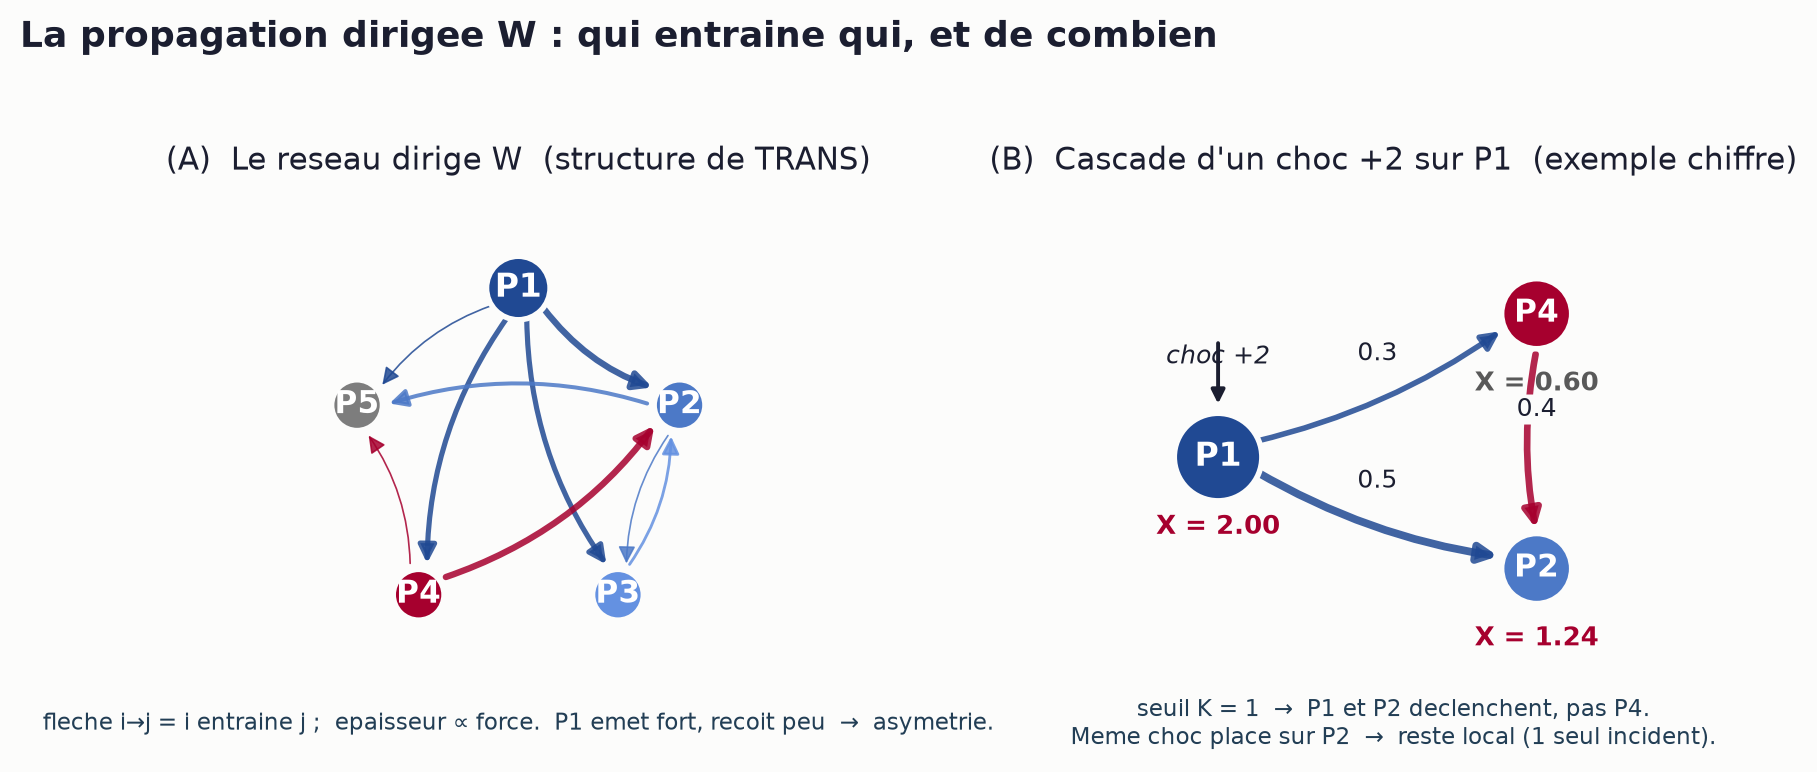
\includegraphics[width=\linewidth]{figures/H1_reseau_W.png}
\caption{(A) La structure dirigée de $W$ sur les 5 piliers : P1 émet fort et reçoit peu.
(B) Le sous-réseau de l'exemple ci-dessous et la propagation d'un choc.}
\end{figure}

\noindent\textbf{Le sous-réseau de l'exemple.} Pour rester vérifiable à la main, on se limite
aux trois piliers $\{$P1, P2, P4$\}$ (ordre des lignes/colonnes : P1, P2, P4). La matrice
dirigée $W$ (\emph{ligne $j$ = ce que le pilier $j$ reçoit}) et son amplificateur de
cascade :
\begin{equation}
W = \begin{pmatrix} 0 & 0 & 0 \\ 0{,}5 & 0 & 0{,}4 \\ 0{,}3 & 0 & 0 \end{pmatrix},
\qquad
(I-W)^{-1} = \begin{pmatrix} 1 & 0 & 0 \\ 0{,}62 & 1 & 0{,}4 \\ 0{,}3 & 0 & 1 \end{pmatrix}.
\end{equation}
P2 reçoit $0{,}5$ de P1 et $0{,}4$ de P4 ; P4 reçoit $0{,}3$ de P1. Le $0{,}62$
vient du chemin direct P1$\to$P2 \emph{plus} le détour P1$\to$P4$\to$P2
($0{,}5 + 0{,}4\times 0{,}3$).

\medskip\noindent\textbf{Un choc systémique $+2$ sur P1 seul}, soit $g=(2,0,0)^\top$, se
propage en
\begin{equation}
X = (I-W)^{-1}\,g = (\,\mathbf{2{,}00}\,;\ \mathbf{1{,}24}\,;\ \mathbf{0{,}60}\,)^\top .
\end{equation}
Avec un seuil $K=1$ : \textbf{P1 et P2 déclenchent} ($X\ge 1$), pas P4. Le choc n'a frappé que
P1, mais la structure dirigée a \emph{propagé} l'incident jusqu'à P2.

\begin{cle}
\textbf{L'asymétrie en un chiffre.} Le \emph{même} choc $+2$ placé sur \textbf{P2}
($g=(0,2,0)^\top$) donne $X=(0\,;\,2\,;\,0)$ : il reste \textbf{local} (P2 n'entraîne personne
ici). Source P1 $\Rightarrow$ \textbf{2 incidents} ; source P2 $\Rightarrow$ \textbf{1 incident}.
C'est exactement l'effet d'ordre du modèle qualitatif, désormais \emph{quantifié} par
$(I-W)^{-1}$.
\end{cle}

\section{Le seuil $K_j$ : ce qui remplace $\Phi^{-1}(\mathrm{PD})$}

\begin{attention}
\textbf{Pourquoi $K_i=\Phi^{-1}(\mathrm{PD}_i)$ tombe en cyber.} La PD n'est pas stable
(la menace évolue), pas mesurable (sous-déclaration), et il n'y a pas de \og{}valeur de firme\fg{}
à franchir. Inverser une gaussienne sur une PD biaisée donne un seuil \textbf{instable et
dénué de sens}. De plus il serait \emph{spécifique à l'entité} et \emph{mobile dans le temps} :
incompatible avec un seuil \emph{global} et \emph{stable}.
\end{attention}

\noindent \textbf{On inverse la logique.} Dans le crédit, la PD est l'entrée et $K$ la sortie.
En cyber, on fixe $K_j$ et la PD devient une \emph{sortie} :
\begin{enumerate}[leftmargin=1.4em,itemsep=2pt]
\item \textbf{Ancrage réglementaire (global + stable).} DORA définit l'\og{}incident majeur\fg{}
  (art.~18 : clients affectés, durée, pertes de données, impact). On prend ce seuil de
  matérialité $u_j$ comme déclencheur : \emph{même définition pour toutes les entités}
  (benchmarking) et \emph{fixée par le règlement} (stable dans le temps).
\item \textbf{Queue calibrée par la théorie des valeurs extrêmes (robuste au biais).}
  Au-dessus de $u_j$, la sévérité suit une loi de Pareto généralisée (GPD). Comme la
  sous-déclaration frappe surtout les \emph{petits} incidents, calibrer la queue sur les
  \emph{gros} (fiablement observés) est robuste. Le seuil devient un seuil EVT, pas
  $\Phi^{-1}$.
\end{enumerate}
La probabilité de dépassement se lit alors comme une \textbf{sortie} du modèle, conditionnelle
à l'état systémique et à la contagion :
\begin{equation}
\pi_{ij}(\mathbf Y) = \mathbb P\big(X_{ij} \ge K_j \mid \mathbf Y\big),\qquad
\mathrm{PD}_j = \mathbb E[\pi_{ij}] = 1 - t_\nu(K_j)\ \ \text{(queue lourde, cf. copule $t$)}.
\end{equation}

\section{Banc d'essai : $\Phi^{-1}(\mathrm{PD})$ contre l'EVT}

On teste numériquement l'argument précédent : sévérités cyber \textbf{à queue lourde} (GPD,
indice $\xi=0{,}40$) avec \textbf{sous-déclaration} des petits incidents ; on compare trois
estimations du capital de queue (VaR~99,5~\%) sur 500 tirages.

\begin{figure}[htbp]\centering
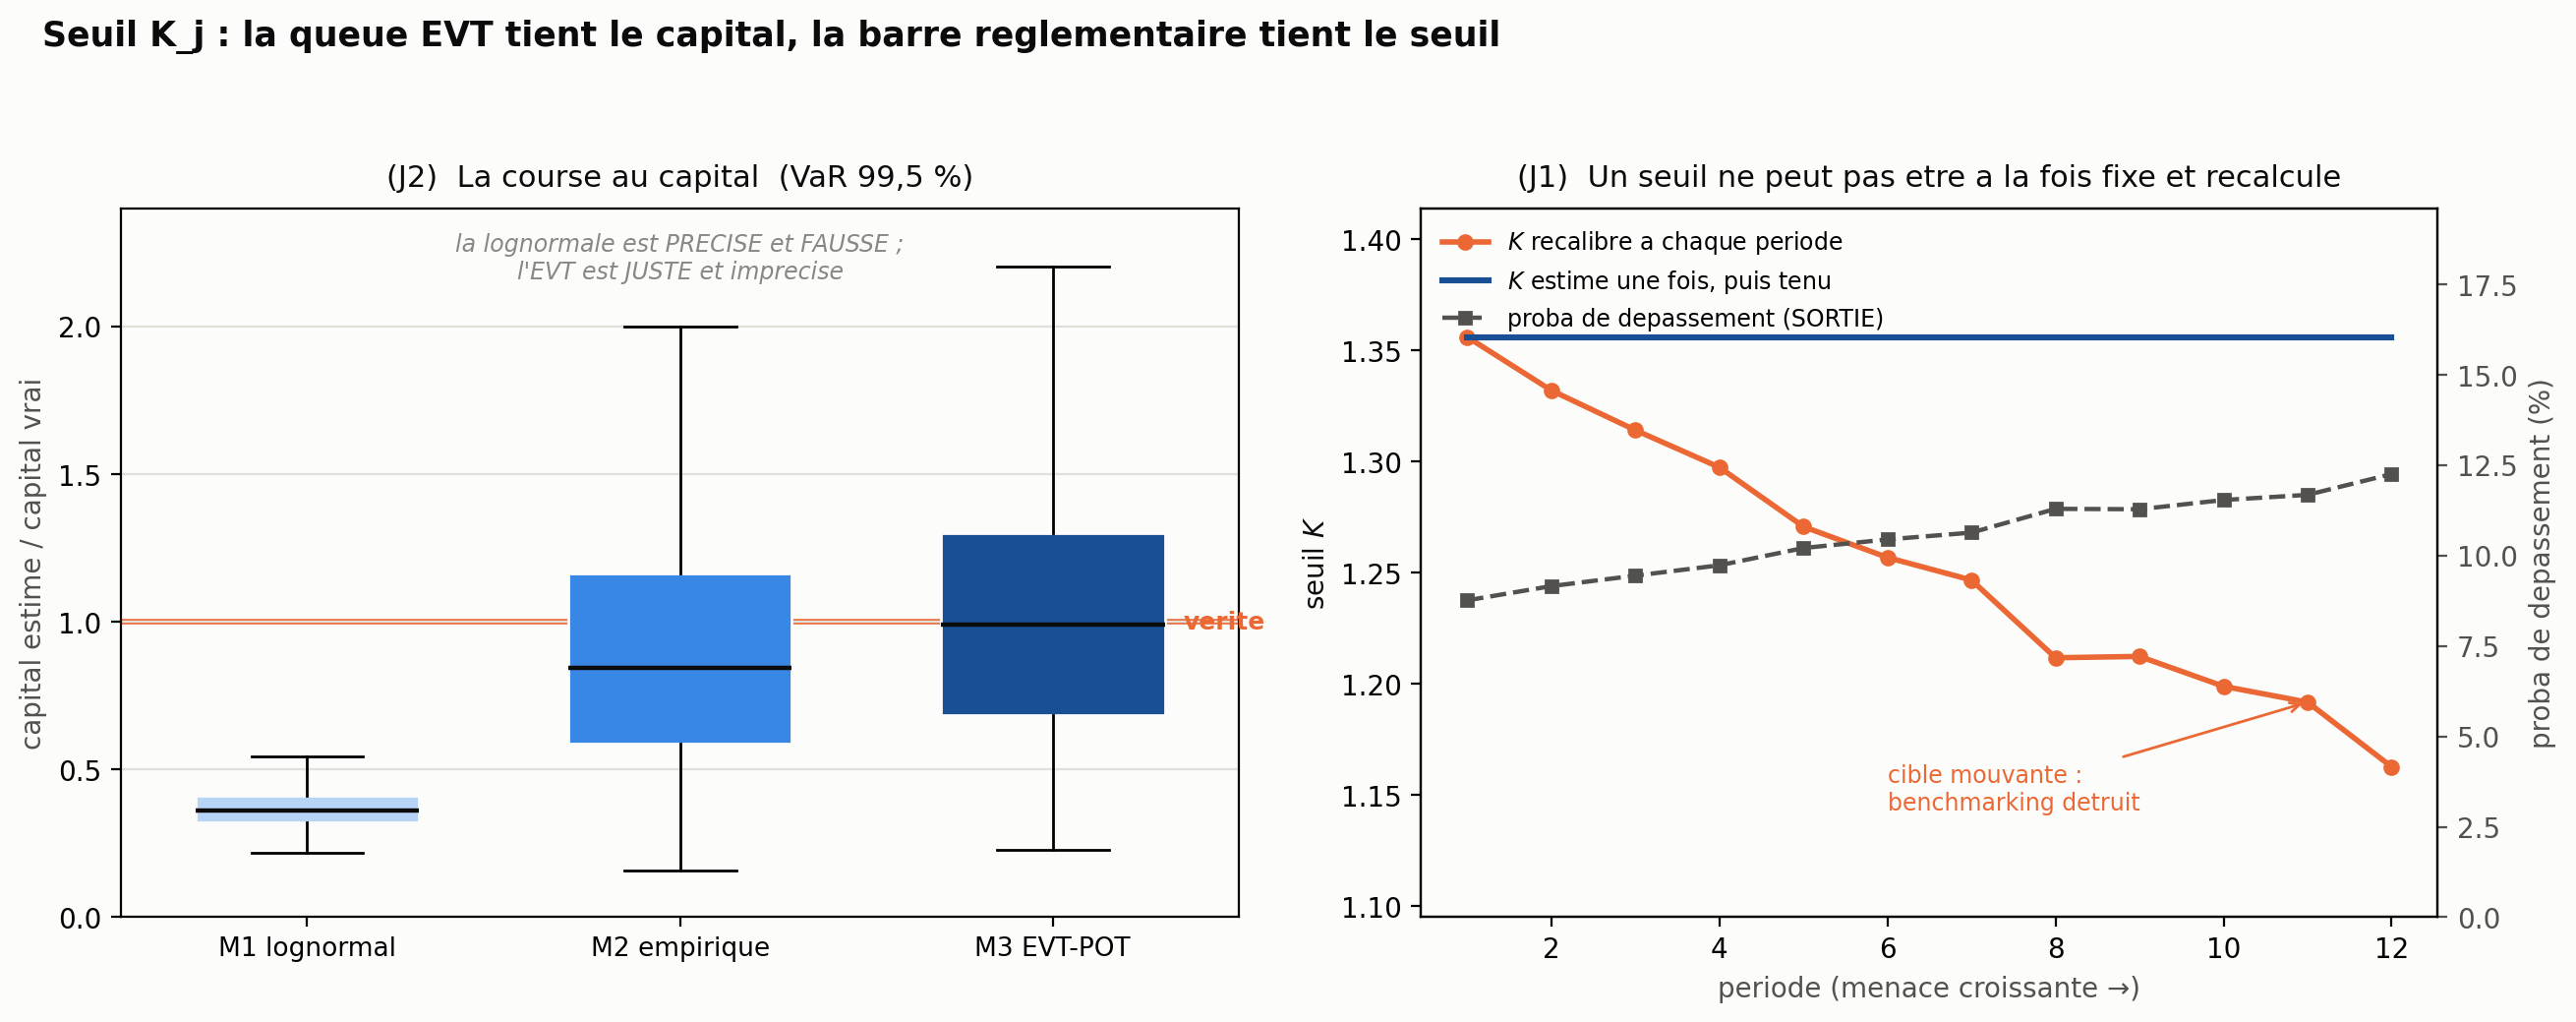
\includegraphics[width=\linewidth]{figures/J_seuil_Ki.png}
\caption{(J2) La lognormale sous-provisionne, l'empirique est instable, l'EVT tombe juste.
(J1) Quand la menace monte, $K=\Phi^{-1}(\mathrm{PD})$ dérive tandis que l'indice de queue EVT
reste stable.}
\end{figure}

\begin{table}[htbp]\centering\small
\renewcommand{\arraystretch}{1.25}
\begin{tabular}{@{}l c l@{}}
\toprule
\textbf{Méthode} & \textbf{Biais médian} & \textbf{Lecture} \\
\midrule
M1 lognormale (monde $\Phi^{-1}$) & $-13{,}6\%$ & sous-provisionne le capital \\
M2 quantile empirique & $-9{,}6\%$ & biaisé \emph{et} très instable \\
M3 EVT / POT & $\mathbf{-1{,}4\%}$ & quasi sans biais \\
\bottomrule
\end{tabular}
\caption{Capital estimé / vérité (VaR~99,5~\%). Vérité $=24{,}1$ unités de perte.}
\end{table}

Deux enseignements robustes :
\begin{itemize}[leftmargin=1.4em,itemsep=1pt]
\item \textbf{Invariance de la queue à la sous-déclaration.} L'indice de queue vaut $0{,}39$
  sur données complètes et $0{,}38$ sur données sous-déclarées (vrai $0{,}40$) : tronquer les
  \emph{petits} incidents ne biaise pas la queue. L'EVT est donc robuste au biais de
  déclaration ; un ajustement lognormal, non.
\item \textbf{Dérive du seuil classique.} $K=\Phi^{-1}(\mathrm{PD})$ passe de $0{,}71$ à
  $0{,}35$ quand la menace monte : cible mouvante, inutilisable comme exigence stable ; l'indice
  de queue EVT reste plat à $0{,}40$.
\end{itemize}

\begin{attention}
\textbf{Portée du banc d'essai.} Les sévérités sont simulées
\emph{déjà} en loi de Pareto : l'EVT ne peut qu'y gagner. Il n'établit donc pas que le
cyber est GPD ; il \textbf{illustre} deux propriétés statistiques \emph{connues} (invariance de
l'indice de queue par troncature à gauche ; instabilité de $\Phi^{-1}(\mathrm{PD})$ sous
non-stationnarité). La défendabilité vient de la \emph{plausibilité du modèle de sévérité
cyber}, pas de ce test.
\end{attention}

\section{Récapitulatif : le modèle en un tableau}

\begin{table}[htbp]\centering\small
\renewcommand{\arraystretch}{1.35}
\begin{tabular}{@{}l l >{\raggedright\arraybackslash}p{5.8cm}@{}}
\toprule
\textbf{Objet} & \textbf{Rôle} & \textbf{Dépend de} \\
\midrule
$\Y_j$ & facteur systémique du pilier & \textbf{du pilier $j$} \\
$\rho_{ij}=\rho_j+u_{ij}$ & sensibilité au systémique & \textbf{de l'entité $i$ et du pilier $j$} (moyenne $\rho_j$) \\
$\Sigma_Y$ & dépendances croisées (symétriques) & des paires de piliers \\
$W_{jk}$ & contagion \textbf{dirigée} $k\to j$ & de l'ordre (asymétrique, TRANS) \\
$\eps_{ij}$ & choc idiosyncratique & de l'entité et du pilier \\
$K_j$ & seuil de déclenchement & \textbf{réglementaire} (DORA), \emph{pas} $\Phi^{-1}(\mathrm{PD})$ \\
\bottomrule
\end{tabular}
\caption{Tout ce qui portait un indice global dans Vasicek devient \textbf{propre au pilier}
ou \textbf{dirigé}. C'est le c\oe ur de l'adaptation à DORA.}
\end{table}

\begin{cle}
\textbf{Synthèse.} \emph{(A)} un facteur systémique \textbf{par pilier} $\Y_j$ et une
sensibilité $\rho_{ij}=\rho_j+u_{ij}$ \textbf{hiérarchique} (moyenne de pilier $\rho_j$ +
écart entité $u_{ij}$) ; \emph{(B)} une contagion \textbf{dirigée} entre piliers ($W$
asymétrique, structure TRANS) ; \emph{(C)} un seuil $K_j$ \textbf{réglementaire} et une queue
\textbf{EVT}, à la place de $\Phi^{-1}(\mathrm{PD})$. Les trois s'emboîtent sur le Vasicek
standard, qu'on retrouve en annulant les extensions.
\end{cle}

\clearpage
\section{Décisions à trancher et données}

Ce modèle ouvre des choix que le mémoire doit \textbf{assumer explicitement}. Les voici, avec
ma recommandation :

\begin{table}[htbp]\centering\small
\renewcommand{\arraystretch}{1.35}
\begin{tabular}{@{}>{\raggedright\arraybackslash}p{3.2cm} >{\raggedright\arraybackslash}p{6.0cm} >{\raggedright\arraybackslash}p{4.9cm}@{}}
\toprule
\textbf{Décision} & \textbf{Options} & \textbf{Recommandation} \\
\midrule
Chargement systémique & $\rho$ global / $\rho_j$ pilier / $\rho_{ij}$ entité & \textbf{hiérarchique} $\rho_{ij}=\rho_j+u_{ij}$ \\
\addlinespace[2pt]
Structure de dépendance & copule gaussienne / Student-$t$ / archimédienne & \textbf{copule $t$} (queue lourde, un seul $\nu$) \\
\addlinespace[2pt]
Seuil $K_j$ & $\Phi^{-1}(\mathrm{PD})$ / matérialité + EVT & \textbf{matérialité DORA + EVT} \\
\addlinespace[2pt]
Contagion $W$ & fixée à dire d'expert / calibrée & à \textbf{estimer} (cf. données) \\
\bottomrule
\end{tabular}
\end{table}

\begin{attention}
\textbf{Le vrai chantier suivant : la donnée.} Tout repose aujourd'hui sur du jugement d'expert
(structure de $W$) et de la simulation. Pour \emph{calibrer} $\rho_j$, $W$ et $\xi$, il faut des
sources réelles :
\begin{itemize}[leftmargin=1.4em,itemsep=1pt,topsep=2pt]
\item \textbf{registres d'incidents DORA} (déclarations obligatoires depuis 2025), la source
  native, mais courte et en montée en charge ;
\item \textbf{rapports ANSSI / ENISA / CERT} pour la fréquence sectorielle ;
\item \textbf{bases publiques} (p.\,ex. notifications RGPD) comme ancrage partiel du biais de
  déclaration.
\end{itemize}
La \textbf{calibration de $W$} (qui entraîne qui, et de combien) est le verrou
méthodologique : sans données, $W$ reste une hypothèse ; avec elles, c'est la \textbf{contribution
empirique} du mémoire.
\end{attention}

\end{document}
